\newpage
\section{Additional Results}

\subsection{Impact of Search Space Resolution}
\begin{figure}[H]
    \centering
    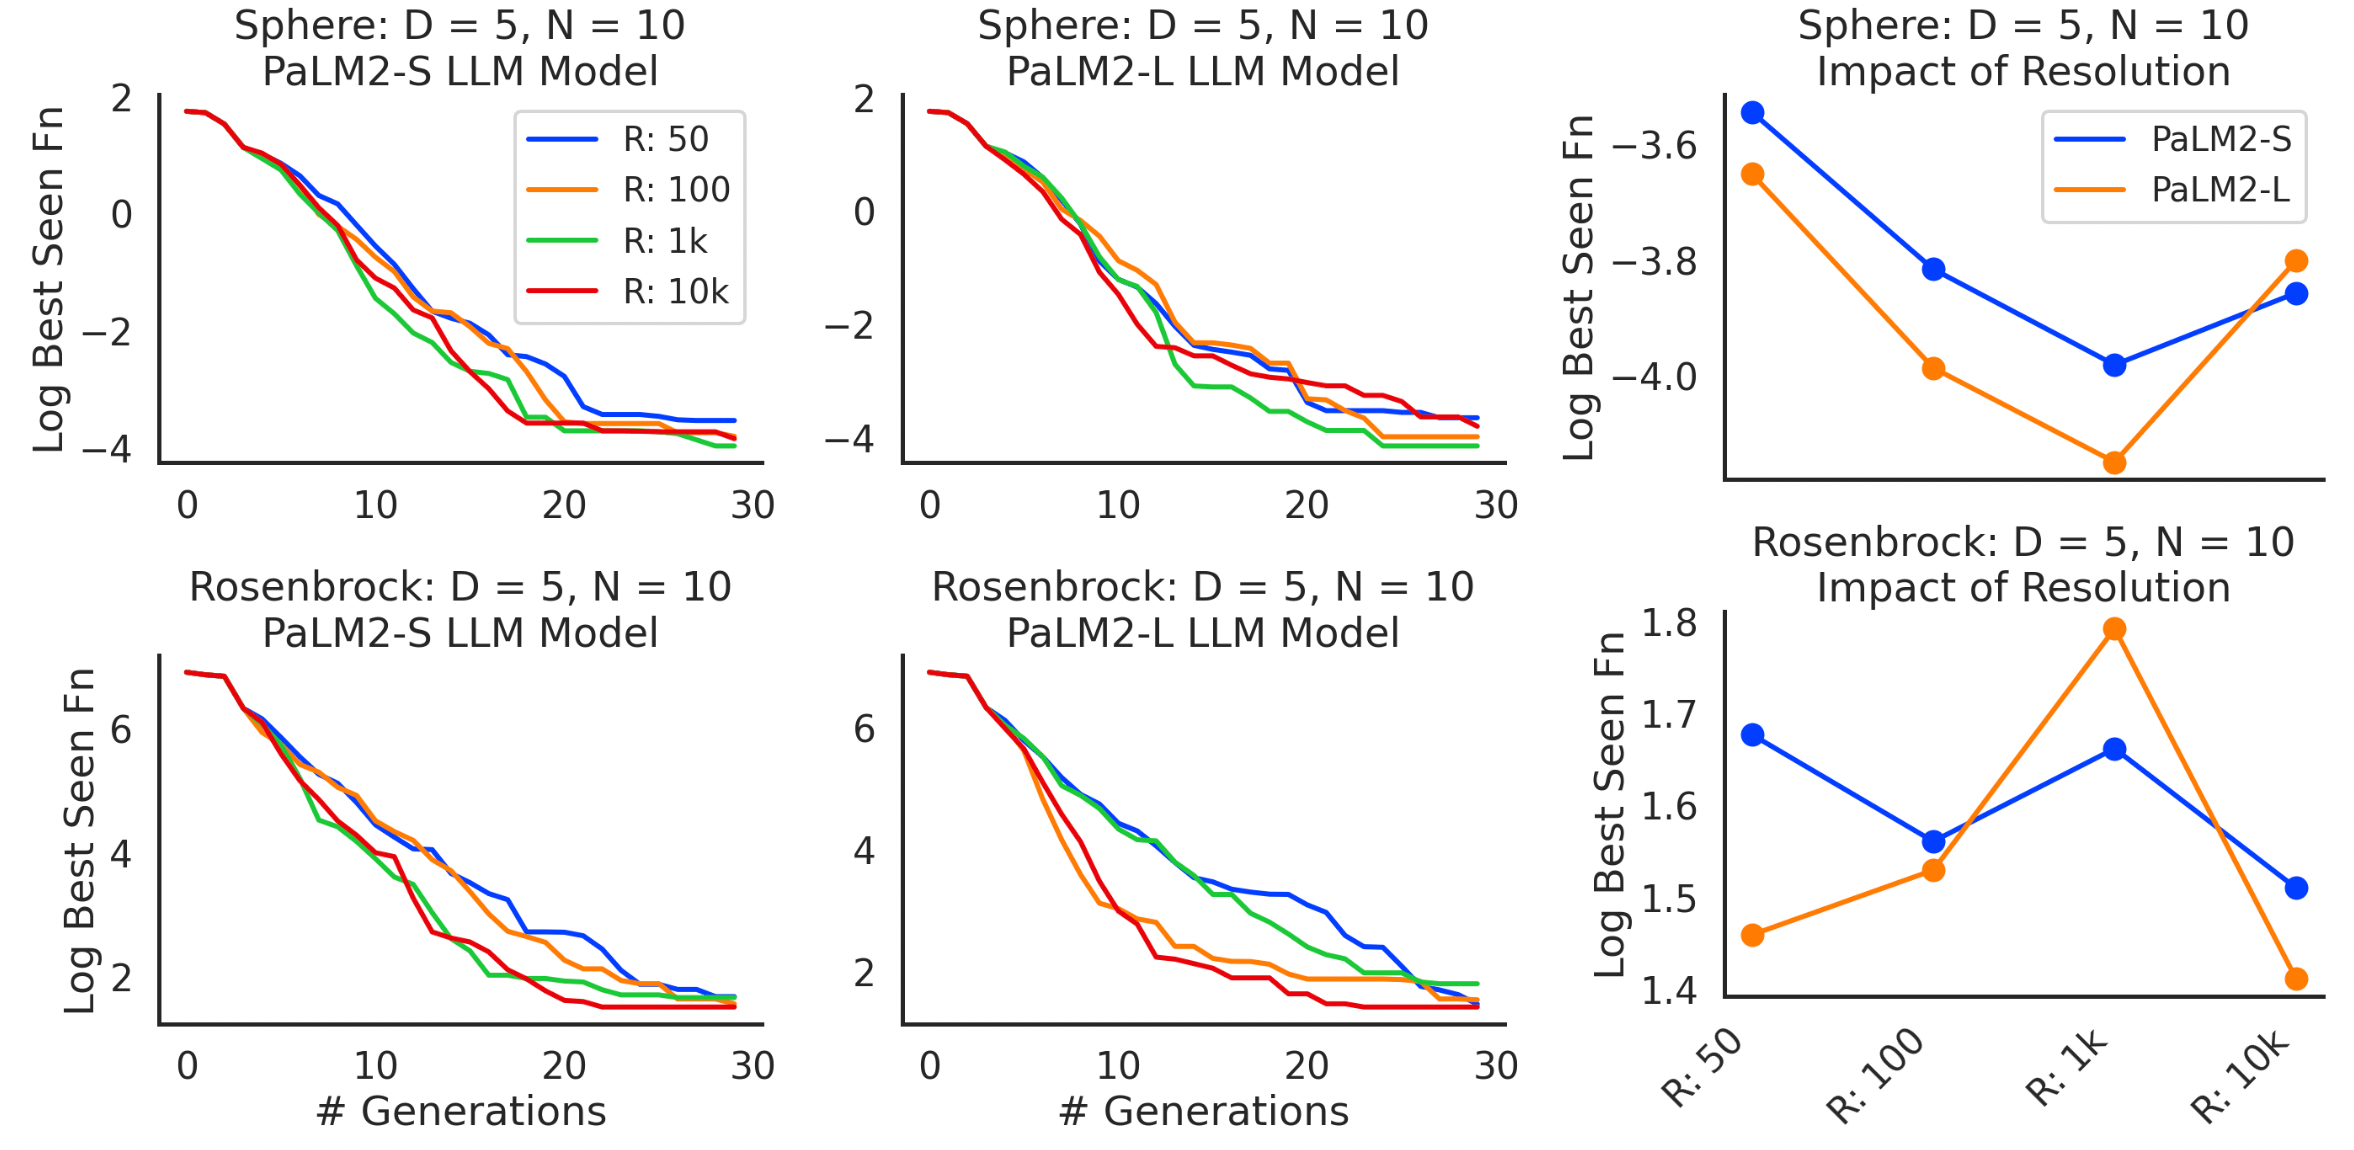
\includegraphics[width=0.475\textwidth]{figures/f8_evollm_resolution.png}
    \caption{EvoLLM performance for different search resolutions. It struggles to zoom into optima basins for low-resolutions, while high resolutions degrade performance due to tokenization. Averaged results over 5 independent runs.}
    \label{fig:results_resolution}
\end{figure}

\subsection{Context Members \& Generations}
\begin{figure}[H]
    \centering
    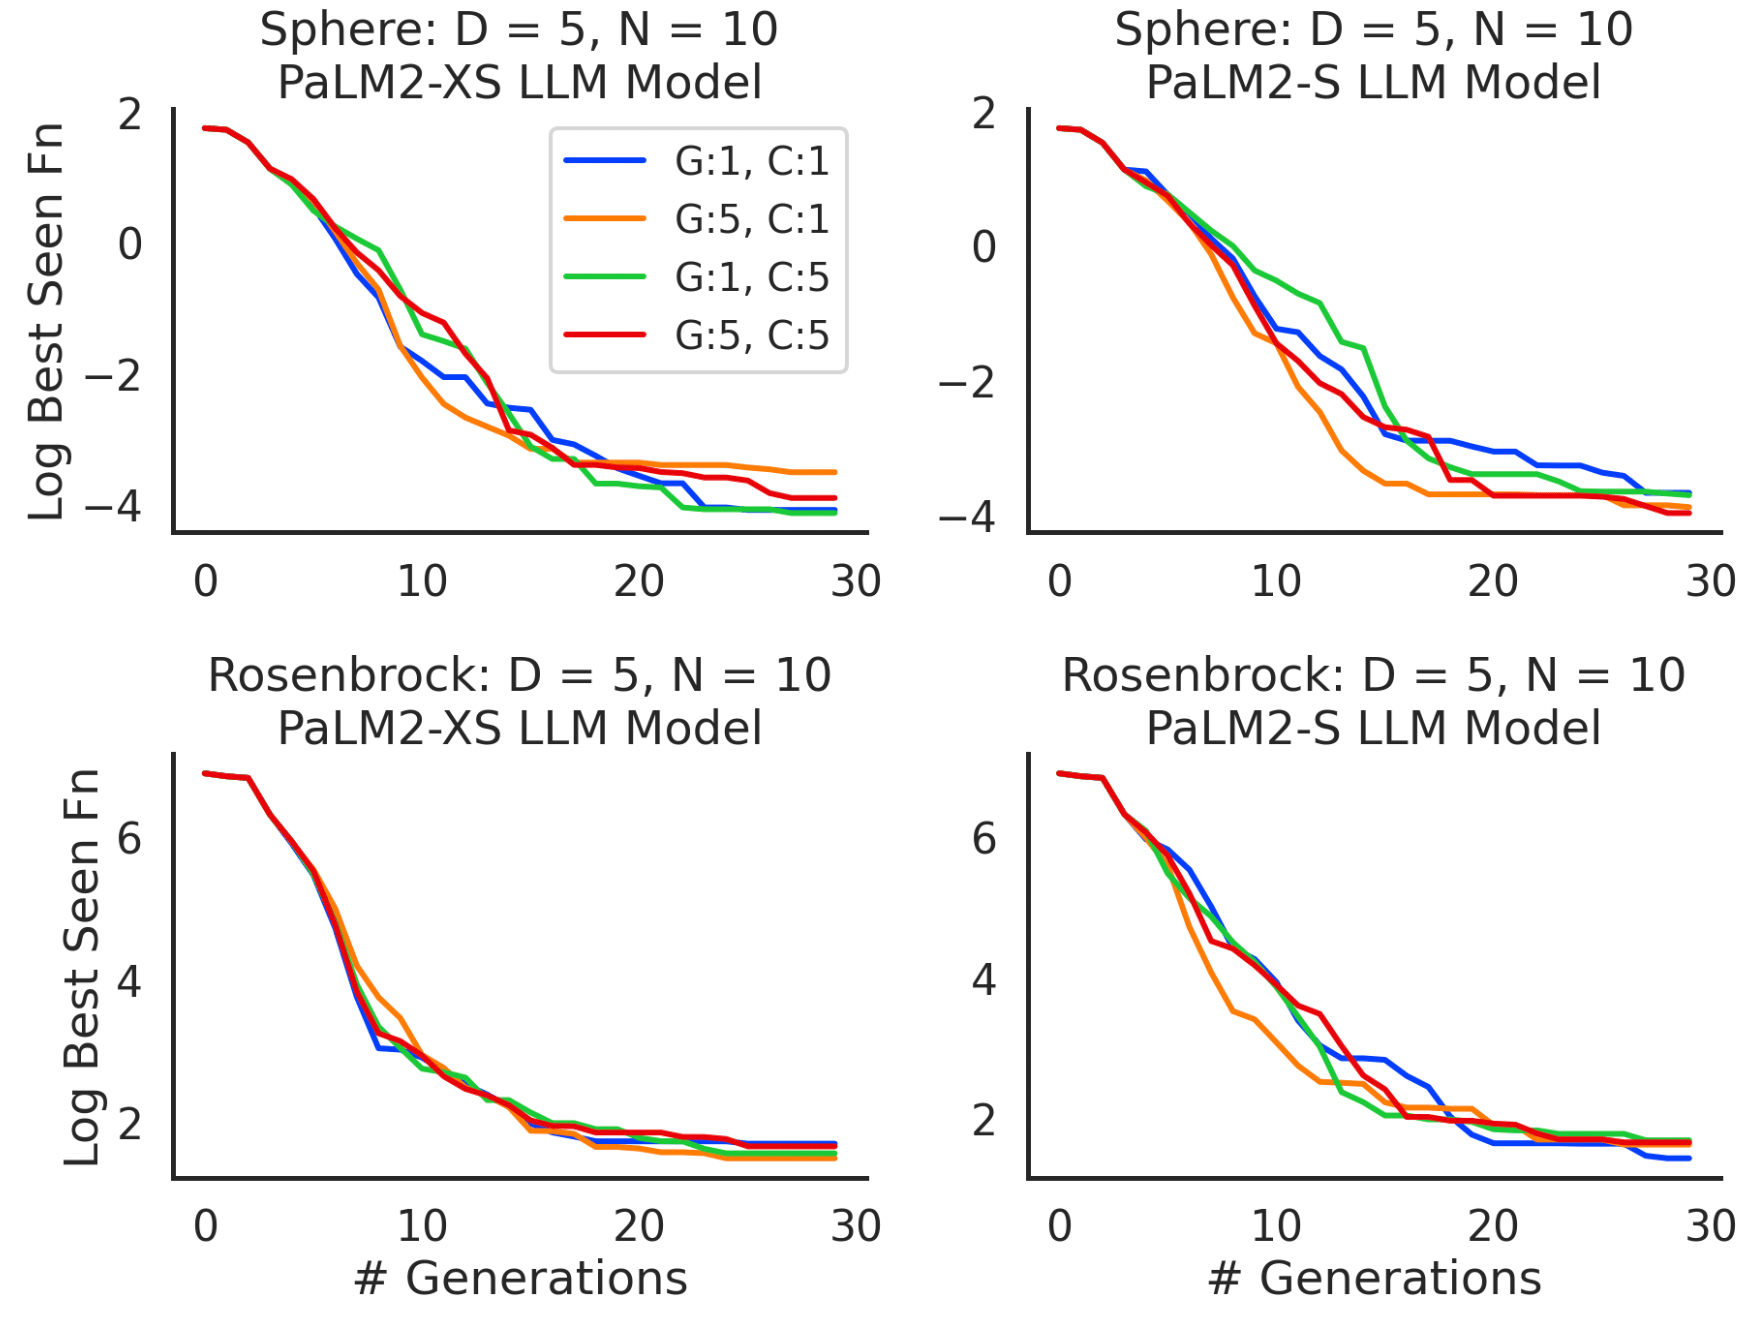
\includegraphics[width=0.45\textwidth]{figures/f9_evollm_context.png}
    \caption{EvoLLM performance for different amounts of context information. Even with limited information the LLM is capable of inferring improving sequence patterns. Averaged results over 5 independent runs.}
    \label{fig:results_context_info}
\end{figure}
%

\section{Prompt Construction Example: 2 Dim. Sphere / 5 Population members}

Below we show an example of the EvoLLM prompt outlined in \cref{table:context_settings} for a 2-dimensional Sphere task with 5 population members. We start with a randomly initialized mean and 4 random search warm-up generations:

% Settings
% context_buffer_settings = dict(
%   max_context_generations=5,  # Number of considered context generations
%   max_context_candidates=5,  # Length of context measured in generations
%   context_generation_setting="last",  # Sample random generations from buffer
%   context_candidate_setting="best-across",  # Permute order of popmembers at construction
%   context_generation_sorting="improving",  # Sort generations worst (top) to best (bottom)
%   context_candidate_sorting="improving",  # Sort candidates worst (right) to best (left)
%   context_generation_unique=False,  # Unique first mean strings across gens
%   max_rel_fitness_progress=0.5,  # Desired fitness improvement between generations
%   use_int_fitness_enc=False,  # Don't use float but int representation
%   use_mean_fitness=False,  # Use mean fitness for scoring in context/prompt
%   use_improvement_bool=True, # Add improvement bool for candidates to prompt
%   use_best_mean=True,  # Use best candidate as mean in context
%   use_log_fitness=False,  # Use log transform of fitness
%   use_fitness_str=True,  # Use fitness string representation
% )
%
% sigma_init = 0.2
% evollm_strategy_kwargs = dict(
%   resolution=1000,
%   lm_model_path= '/sax/yujintang/ulm8b_hillclimber', #'text-davinci-003', # '/sax/yujintang/ulm24b', #
%   temperature=(0.2, 0.6, 0.8, 1.0),
%   max_decode_steps=None,
%   warm_up_strategy="RandomSearch",
%   warm_up_generations=4,  # Warm-up generations with BBO algorithm
%   warm_up_seed=0,
%   context_buffer_settings=context_buffer_settings,
%   fix_seed=True,
%   verbose=True,
% )
%
$\mu = [ 2.93851025 -1.77656265], f^\star = 0.4378929557544995$ 
\newpage
================ Generation 0 ================= \\
\begin{empheq}[box=\mymath]{align*}
\scriptstyle
&0.44: 397 539;147 92,0,0 302,0,186 346,0,419 685,0,397 539,0\\
&0.39: \Rightarrow \mu = [-0.61939515  0.2329004 ], \ f^\star = 0.438
\end{empheq}
================ Generation 1 =================\\
\begin{empheq}[box=\mymath]{align*}
&1.29: 397 539;559 140,0,186 346,0,419 685,0,670 417,0,397 539,0 \\
&0.44: 397 539;147 92,0,0 302,0,186 346,0,419 685,0,397 539,0 \\
&0.29: \Rightarrow \mu = [-0.61939515  0.2329004 ], \ f^\star = 0.438 
\end{empheq}
================ Generation 2 =================\\
\begin{empheq}[box=\mymath]{align*}
&6.03: 397 539;559 140,0,186 346,0,419 685,0,670 417,0,397 539,0 \\
&1.29: 397 539;559 140,0,186 346,0,419 685,0,670 417,0,397 539,0 \\
&0.44: 397 539;147 92,0,0 302,0,186 346,0,419 685,0,397 539,0 \\
&0.29: \Rightarrow  \mu = [-0.61939515  0.2329004 ], \ f^\star = 0.438
\end{empheq}
================ Generation 3 ================= \\
\begin{empheq}[box=\mymath]{align*}
&6.03: 397 539;559 140,0,186 346,0,419 685,0,670 417,0,397 539,0 \\
&2.48: 397 539;748 280,0,316 687,0,419 685,0,670 417,0,397 539,0 \\
&1.29: 397 539;559 140,0,186 346,0,419 685,0,670 417,0,397 539,0 \\
&0.44: 397 539;147 92,0,0 302,0,186 346,0,419 685,0,397 539,0 \\
&0.34: \Rightarrow  \mu = [-0.618  0.234], \ f^\star = 0.339
\end{empheq}
================ Generation 4 ================= \\
\begin{empheq}[box=\mymath]{align*}
&6.03: 397 539;559 140,0,186 346,0,419 685,0,670 417,0,397 539,0\\
&2.48: 397 539;748 280,0,316 687,0,419 685,0,670 417,0,397 539,0\\
&1.29: 397 539;559 140,0,186 346,0,419 685,0,670 417,0,397 539,0\\
&0.44: 397 539;147 92,0,0 302,0,186 346,0,419 685,0,397 539,0\\
&0.34: 413 543;388 557,0,448 604,0,397 539,0,399 504,1,413 543,1\\
&0.25: \Rightarrow \mu = [-0.522  0.258], \ f^\star = 0.249
\end{empheq}
================ Generation 5 ================= \\
\begin{empheq}[box=\mymath]{align*}
&6.03: 397 539;559 140,0,186 346,0,419 685,0,670 417,0,397 539,0 \\
&2.48: 397 539;748 280,0,316 687,0,419 685,0,670 417,0,397 539,0 \\
&1.29: 397 539;559 140,0,186 346,0,419 685,0,670 417,0,397 539,0 \\
&0.34: 413 543;388 557,0,448 604,0,397 539,0,399 504,1,413 543,1 \\
&0.25: 423 531;417 564,0,399 504,0,413 543,0,415 522,1,423 531,1 \\
&0.20: \Rightarrow \mu = [-0.462  0.186], \ f^\star = 0.15
\end{empheq}
================ Generation 6 ================= \\
\begin{empheq}[box=\mymath]{align*}
&6.03: 397 539;559 140,0,186 346,0,419 685,0,670 417,0,397 539,0 \\
&2.48: 397 539;748 280,0,316 687,0,419 685,0,670 417,0,397 539,0 \\
&0.34: 413 543;388 557,0,448 604,0,397 539,0,399 504,1,413 543,1\\
&0.25: 423 531;417 564,0,399 504,0,413 543,0,415 522,1,423 531,1\\
&0.15: 436 506;413 543,0,415 522,0,423 531,0,487 564,1,436 506,1\\
&0.09: \Rightarrow \mu = [-0.384  0.036], \ f^\star = 0.101
\end{empheq}
================ Generation 7 ================= \\
\begin{empheq}[box=\mymath]{align*}
&2.48: 397 539;748 280,0,316 687,0,419 685,0,670 417,0,397 539,0 \\
&0.34: 413 543;388 557,0,448 604,0,397 539,0,399 504,1,413 543,1 \\
&0.25: 423 531;417 564,0,399 504,0,413 543,0,415 522,1,423 531,1 \\
&0.15: 436 506;413 543,0,415 522,0,423 531,0,487 564,1,436 506,1 \\
&0.10: 447 499;434 527,0,487 564,0,436 506,0,439 514,1,447 499,1 \\
&0.07: \Rightarrow \mu = [-0.318 -0.006], \ f^\star = 0.040
\end{empheq}
================ Generation 8 ================= \\
\begin{empheq}[box=\mymath]{align*}
&0.34: 413 543;388 557,0,448 604,0,397 539,0,399 504,1,413 543,1 \\
&0.25: 423 531;417 564,0,399 504,0,413 543,0,415 522,1,423 531,1 \\
&0.15: 436 506;413 543,0,415 522,0,423 531,0,487 564,1,436 506,1 \\
&0.10: 447 499;434 527,0,487 564,0,436 506,0,439 514,1,447 499,1 \\
&0.04: 472 481;436 506,0,439 514,0,442 500,0,447 499,0,472 481,1 \\
&0.03: \Rightarrow \mu = [-0.168 -0.114], \ f^\star = 0.018
\end{empheq}
================ Generation 9 ================= \\
\begin{empheq}[box=\mymath]{align*}
&0.25: 423 531;417 564,0,399 504,0,413 543,0,415 522,1,423 531,1 \\
&0.15: 436 506;413 543,0,415 522,0,423 531,0,487 564,1,436 506,1 \\
&0.10: 447 499;434 527,0,487 564,0,436 506,0,439 514,1,447 499,1 \\
&0.04: 472 481;436 506,0,439 514,0,442 500,0,447 499,0,472 481,1 \\
&0.02: 478 495;465 474,0,472 481,0,476 519,1,479 485,1,478 495,1 \\
&0.01: \Rightarrow \mu = [-0.132 -0.03 ], \ f^\star = 0.018
\end{empheq}
================ Generation 10 ================= \\
\begin{empheq}[box=\mymath]{align*}
&0.15: 436 506;413 543,0,415 522,0,423 531,0,487 564,1,436 506,1 \\
&0.10: 447 499;434 527,0,487 564,0,436 506,0,439 514,1,447 499,1 \\
&0.05: 478 495;483 467,0,472 481,0,476 519,0,479 485,0,478 495,0 \\
&0.04: 472 481;436 506,0,439 514,0,442 500,0,447 499,0,472 481,1 \\
&0.02: 478 495;465 474,0,472 481,0,476 519,1,479 485,1,478 495,1 \\
&0.01: \Rightarrow \mu = [-0.132 -0.03 ], \ f^\star = 0.018
\end{empheq}

% ==================== Gen 11 ====================
% 0.10: 447 499;434 527,0,487 564,0,436 506,0,439 514,1,447 499,1
% 0.05: 478 495;483 467,0,472 481,0,476 519,0,479 485,0,478 495,0
% 0.04: 472 481;436 506,0,439 514,0,442 500,0,447 499,0,472 481,1
% 0.02: 478 495;472 481,0,476 519,0,479 485,0,480 511,0,478 495,0
% 0.02: 478 495;465 474,0,472 481,0,476 519,1,479 485,1,478 495,1
% 0.01: 
% -> [-0.132 -0.03 ] 0.01810261965231823
% ==================== Gen 12 ====================
% 0.05: 478 495;483 467,0,472 481,0,476 519,0,479 485,0,478 495,0
% 0.04: 472 481;436 506,0,439 514,0,442 500,0,447 499,0,472 481,1
% 0.03: 478 495;472 514,0,476 519,0,479 485,0,480 511,0,478 495,0
% 0.02: 478 495;472 481,0,476 519,0,479 485,0,480 511,0,478 495,0
% 0.02: 478 495;465 474,0,472 481,0,476 519,1,479 485,1,478 495,1
% 0.02: 
% -> [-0.132 -0.03 ] 0.01810261965231823
% ==================== Gen 13 ====================
% 0.05: 478 495;483 467,0,472 481,0,476 519,0,479 485,0,478 495,0
% 0.03: 478 495;472 514,0,476 519,0,479 485,0,480 511,0,478 495,0
% 0.02: 478 495;476 519,0,504 474,0,479 485,0,480 511,0,478 495,0
% 0.02: 478 495;472 481,0,476 519,0,479 485,0,480 511,0,478 495,0
% 0.02: 478 495;465 474,0,472 481,0,476 519,1,479 485,1,478 495,1
% 0.02: 
% -> [-0.132 -0.03 ] 0.011081820194094469
% ==================== Gen 14 ====================
% 0.05: 478 495;483 467,0,472 481,0,476 519,0,479 485,0,478 495,0
% 0.03: 478 495;472 514,0,476 519,0,479 485,0,480 511,0,478 495,0
% 0.02: 478 495;476 519,0,504 474,0,479 485,0,480 511,0,478 495,0
% 0.02: 478 495;472 481,0,476 519,0,479 485,0,480 511,0,478 495,0
% 0.01: 517 504;504 474,0,479 485,0,480 511,0,478 495,0,517 504,1
% 0.01: 
% -> [0.102 0.024] 0.011081820194094469
% ==================== Gen 15 ====================
% 0.03: 478 495;472 514,0,476 519,0,479 485,0,480 511,0,478 495,0
% 0.03: 517 504;504 474,0,479 485,0,480 511,0,478 495,0,517 504,0
% 0.02: 478 495;476 519,0,504 474,0,479 485,0,480 511,0,478 495,0
% 0.02: 478 495;472 481,0,476 519,0,479 485,0,480 511,0,478 495,0
% 0.01: 517 504;504 474,0,479 485,0,480 511,0,478 495,0,517 504,1
% 0.01: 
% -> [0.102 0.024] 0.0010828582819066162
% ==================== Gen 16 ====================
% 0.03: 478 495;472 514,0,476 519,0,479 485,0,480 511,0,478 495,0
% 0.03: 517 504;504 474,0,479 485,0,480 511,0,478 495,0,517 504,0
% 0.02: 478 495;476 519,0,504 474,0,479 485,0,480 511,0,478 495,0
% 0.01: 517 504;504 474,0,479 485,0,480 511,0,478 495,0,517 504,1
% 0.00: 496 497;479 485,0,480 511,0,478 495,0,517 504,0,496 497,1
% 0.00: 
% -> [-0.024 -0.018] 0.0010828582819066162
% ==================== Gen 17 ====================
% 0.03: 517 504;504 474,0,479 485,0,480 511,0,478 495,0,517 504,0
% 0.02: 478 495;476 519,0,504 474,0,479 485,0,480 511,0,478 495,0
% 0.01: 517 504;504 474,0,479 485,0,480 511,0,478 495,0,517 504,1
% 0.00: 496 497;480 511,0,478 495,0,517 504,0,497 489,0,496 497,0
% 0.00: 496 497;479 485,0,480 511,0,478 495,0,517 504,0,496 497,1
% 0.00: 
% -> [-0.024 -0.018] 0.0010828582819066162
% ==================== Gen 18 ====================
% 0.03: 517 504;504 474,0,479 485,0,480 511,0,478 495,0,517 504,0
% 0.02: 496 497;478 495,0,483 515,0,517 504,0,497 489,0,496 497,0
% 0.01: 517 504;504 474,0,479 485,0,480 511,0,478 495,0,517 504,1
% 0.00: 496 497;480 511,0,478 495,0,517 504,0,497 489,0,496 497,0
% 0.00: 496 497;479 485,0,480 511,0,478 495,0,517 504,0,496 497,1
% 0.00: 
% -> [-0.024 -0.018] 0.0010828582819066162
% ==================== Gen 19 ====================
% 0.03: 517 504;504 474,0,479 485,0,480 511,0,478 495,0,517 504,0
% 0.02: 496 497;478 495,0,483 515,0,517 504,0,497 489,0,496 497,0
% 0.00: 496 497;480 511,0,478 495,0,517 504,0,497 489,0,496 497,0
% 0.00: 496 497;510 516,0,517 504,0,497 489,0,498 508,0,496 497,0
% 0.00: 496 497;479 485,0,480 511,0,478 495,0,517 504,0,496 497,1
% 0.00: 
% -> [-0.024 -0.018] 0.0010828582819066162
% ==================== Gen 20 ====================
% 0.02: 496 497;478 495,0,483 515,0,517 504,0,497 489,0,496 497,0
% 0.01: 496 497;517 504,0,484 497,0,497 489,0,498 508,0,496 497,0
% 0.00: 496 497;480 511,0,478 495,0,517 504,0,497 489,0,496 497,0
% 0.00: 496 497;510 516,0,517 504,0,497 489,0,498 508,0,496 497,0
% 0.00: 496 497;479 485,0,480 511,0,478 495,0,517 504,0,496 497,1
% 0.00: 

\newpage
\section{Floating Point Number Tokenization}

Below we show that the number of tokens used for a floating pointing number linearly increases with the number of digits. The numbers are sampled randomly:

\begin{figure}[H]
    \centering
    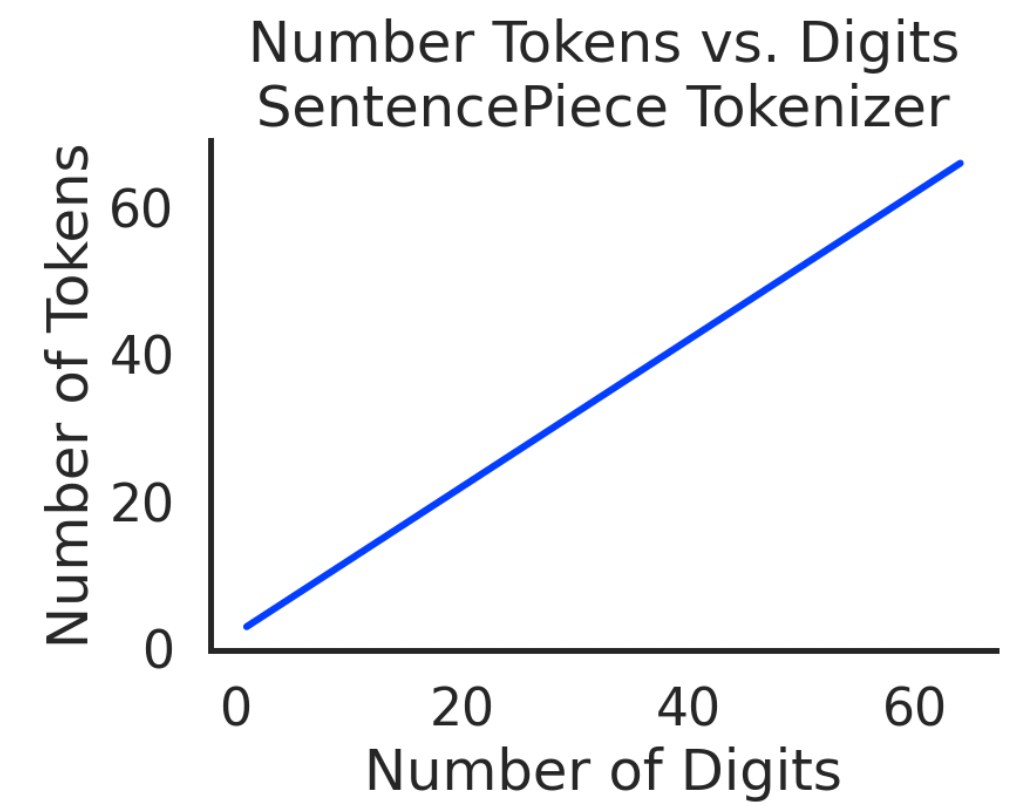
\includegraphics[width=0.35\textwidth]{figures/f_supp_tokenizer.png}
    \caption{SentencePiece Tokenizer floating point number digits versus resulting tokens used for the language model.}
    \label{fig:supp_tokenizer}
\end{figure}

\section{Hill Climbing Instruction Fine-Tuning}

\begin{figure}[H]
    \centering
    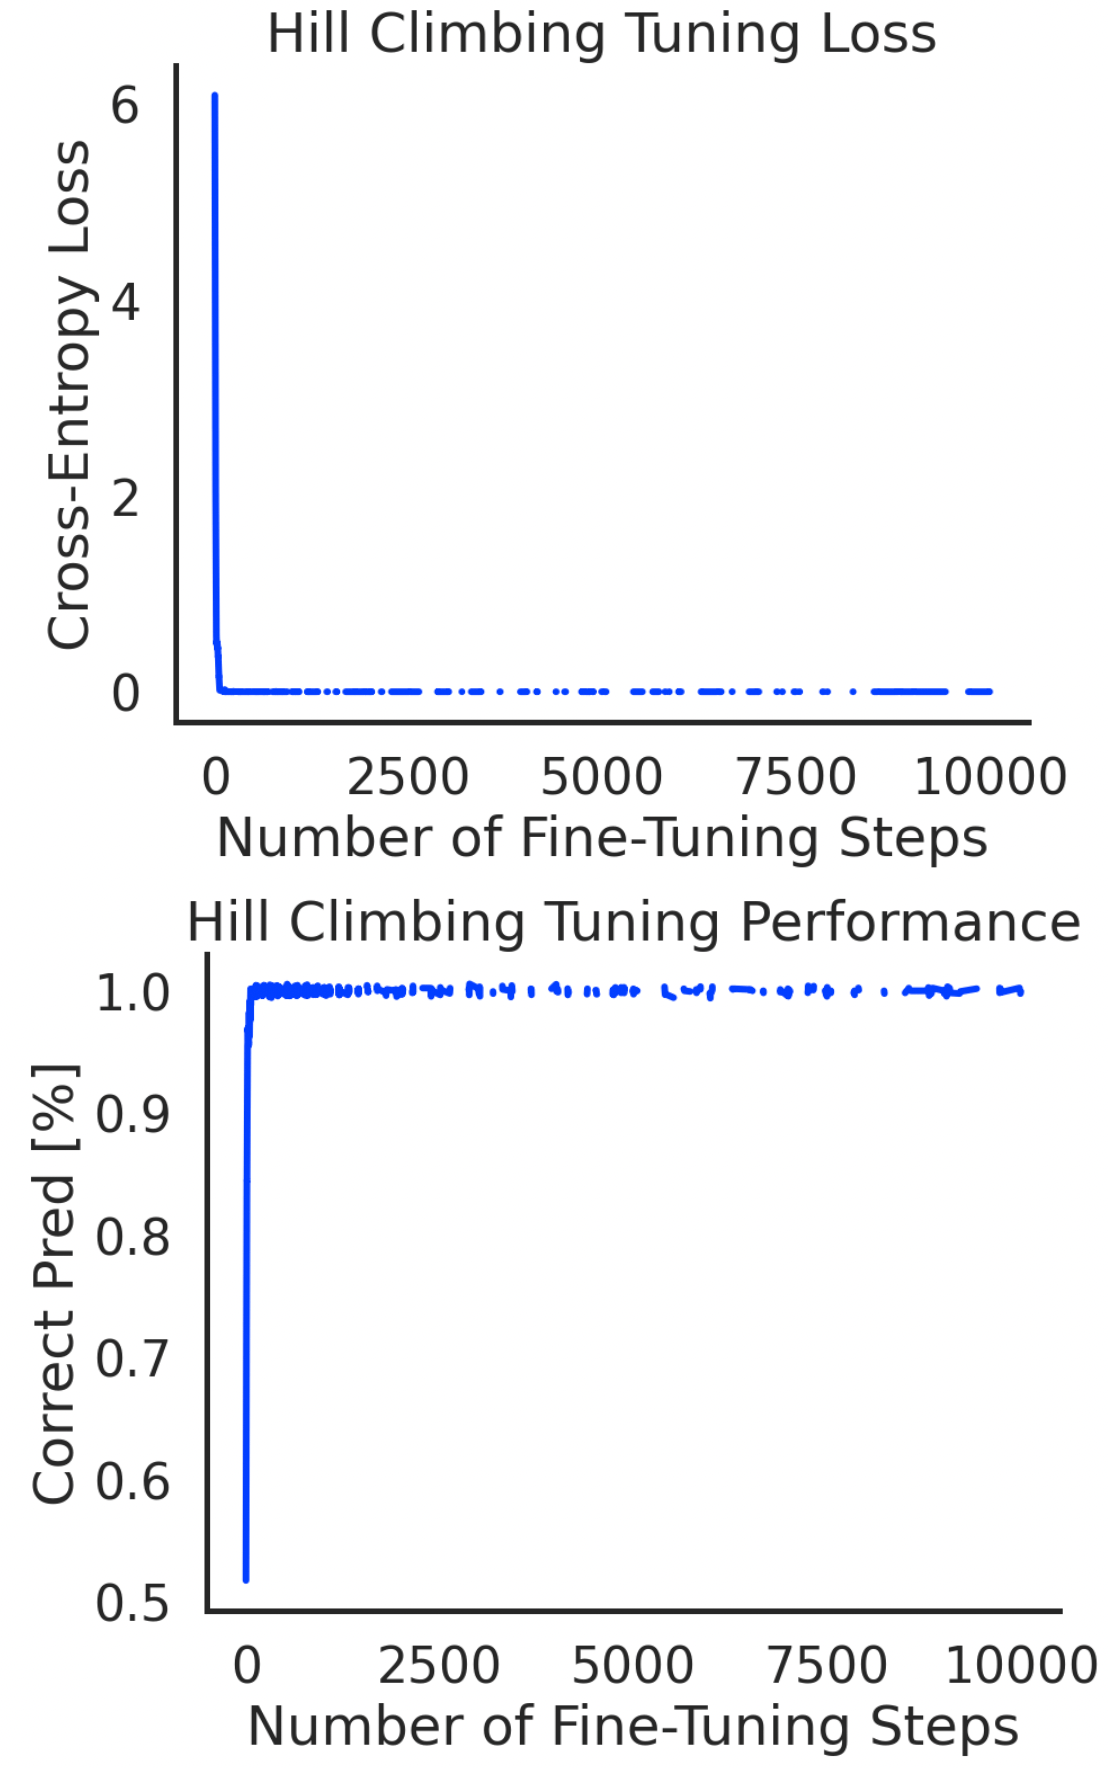
\includegraphics[width=0.35\textwidth]{figures/f_supp_ftune.png}
    \caption{Fine-tuning loss and accuracy for instruction fine-tuning using Hill Climbing teacher algorithm trajectories on PaLM-XS.}
    \label{fig:supp_ftune}
\end{figure}

% \begin{figure*}[h]
% \centering
% \includegraphics[width=0.85\textwidth]{figures/f3_pop_detail.png}%
% \caption{Comparison of different ES (OpenAI-ES, PGPE, SNES and Sep-CMA-ES) across population sizes on four continuous control tasks. The results are averaged over 3 independent runs and we report one standard deviation bars.}
% \label{fig3:details}
% \end{figure*}

% \section*{Acknowledgments}

% We thank Yujin Tang, Yingtao Tian and Chris Lu for constructive discussions. This work is funded by the Deutsche Forschungsgemeinschaft (DFG, German Research Foundation) under Germany’s Excellence Strategy - EXC 2002/1 “Science of Intelligence” - project number 390523135. RTL was additionally supported by a Google Cloud Research Credit Grant.
% Simulations were conducted on a high-performance cluster and were organized using the \texttt{MLE-Infrastructure} \citep[MIT license]{mle_infrastructure2021github} training management system. 



% \newpage
% \appendix
% \vspace{-0.15cm}
% \section{Software \& Compute Requirements}

% Simulations were conducted on a high-performance cluster using three independent runs (random seeds). Depending on the setting, a single run lasts between 30 minutes and 4 hours of training time on a single V100S. Experiments were organized using the \texttt{MLE-Infrastructure} \citep[MIT license]{mle_infrastructure2021github} training management system. 

% \vspace{-0.15cm}
% \section{Brax-Task Hyperparameters}

% \begin{table}[H]
% \centering
% \small
% \begin{tabular}{|r|l||r|l|}
% \hline \hline
% Parameter & Value & Parameter & Value \\ 
% \hline
% Population Size                & 256   & \# Generations        & 2000      \\
% Episode Env Steps                & 1000   & \# Train MC Rollouts        & 16      \\
% Evaluate Every Gens                & 25   & \# Test MC Rollouts        & 128      \\
% Network Type                & MLP   & \# Hidden Units        & 32      \\
% Hidden Activation           & Tanh   & \# Hidden Layers        & 4      \\
% Output Activation           & Tanh   & \# Total Params        & 6248      \\
% \hline \hline
% \end{tabular}
% \caption{Shared hyperparameters for Brax \citep{freeman2021brax} control tasks.}
% \end{table}

% \vspace{-1.05cm}

% \begin{table}[H]
% \centering
% \small
% \begin{tabular}{|r|l|r|l|r|}
% \hline \hline
% Parameter & Ant & Fetch & HalfCheetah & Humanoid \\ 
% \hline
% Sigma init                 & 0.05   &   0.125      & 0.05 & 0.1      \\
% Elite ratio                & 0.4   &     0.2    & 0.5 & 0.2      \\
% \hline \hline
% \end{tabular}
% \caption{Hyperparameters for Sep-CMA-ES \citep{ros2008simple}.}
% \end{table}

% \vspace{-1.15cm}

% \begin{table}[H]
% \centering
% \small
% \begin{tabular}{|r|l|r|l|r|}
% \hline \hline
% Parameter & Ant & Fetch & HalfCheetah & Humanoid \\ 
% \hline
% Lrate init                & 0.01   &    0.02     & 0.01  &    0.02\\
% -- decay                & 0.999   &    0.999     & 0.999    &  0.999\\
% -- final                & 0.001   &  0.001       & 0.001      & 0.001\\
% Sigma init                & 0.05   &   0.05      & 0.075   &   0.1\\
% -- decay                & 0.999   &   0.999      & 0.999    & 0.999 \\
% -- final                & 0.01   &    0.01     & 0.01    &  0.01\\
% Optimizer                & Adam   &    Adam     & Adam & Adam    \\
% Fitness shaping                & Cent. rank   &    Cent. rank     & Cent. rank   & Cent. rank  \\
% \hline \hline
% \end{tabular}
% \caption{Hyperparameters for OpenAI-ES \citep{salimans2017evolution}.}
% \end{table}

% \vspace{-1.05cm}

% \begin{table}[H]
% \centering
% \small
% \begin{tabular}{|r|l|r|l|r|}
% \hline \hline
% Parameter & Ant & Fetch & HalfCheetah & Humanoid \\ 
% \hline
% Lrate init                & 0.01   &    0.02     & 0.02    & 0.02 \\
% -- decay                & 0.999   &     0.999    & 0.999     & 0.999\\
% -- final                & 0.001   &   0.001      & 0.001    &  0.001\\
% Sigma init                & 0.025   &   0.05      & 0.025     & 0.05\\
% -- decay                & 0.999   &   0.999      & 0.999     & 0.999 \\
% -- final                & 0.01   &     0.01    & 0.01     & 0.01\\
% -- learning rate & 0.2 & 0.2& 0.2& 0.2\\
% -- max. change & 0.2 & 0.2 & 0.2 & 0.2\\
% Optimizer                & Adam   &    Adam     & Adam & Adam    \\
% Fitness shaping                & Cent. rank   &    Cent. rank     & Cent. rank   & Cent. rank  \\
% \hline \hline
% \end{tabular}
% \caption{Hyperparameters for PGPE \citep{sehnke2010parameter}.}
% \end{table}

% \vspace{-1.05cm}

% \begin{table}[H]
% \centering
% \small
% \begin{tabular}{|r|l|r|l|r|}
% \hline \hline
% Parameter & Ant & Fetch & HalfCheetah & Humanoid \\ 
% \hline
% Sigma init                & 0.05   &     0.075    & 0.05  & 0.075\\
% $\beta$ Temperature                & 12   &     12    &  16 & 32      \\
% \hline \hline
% \end{tabular}
% \caption{Hyperparameters for SNES \citep{wierstra2014natural}.}
% \end{table}

% \vspace{-0.5cm}
% SNES uses the following utility/fitness shaping transformation:
% \vspace{-0.1cm}
% \begin{equation*}
%     \boldsymbol{w}_{t, j} = \text{softmax}\left(\beta \times \left(\text{rank}(j)/N - 0.5 \right)\right), \ \forall j=1,..., N.
% \end{equation*}


% https://arxiv.org/pdf/2308.11432.pdf